\documentclass{standalone}

\usepackage{tikz}
\usetikzlibrary{shapes.geometric}
\begin{document}
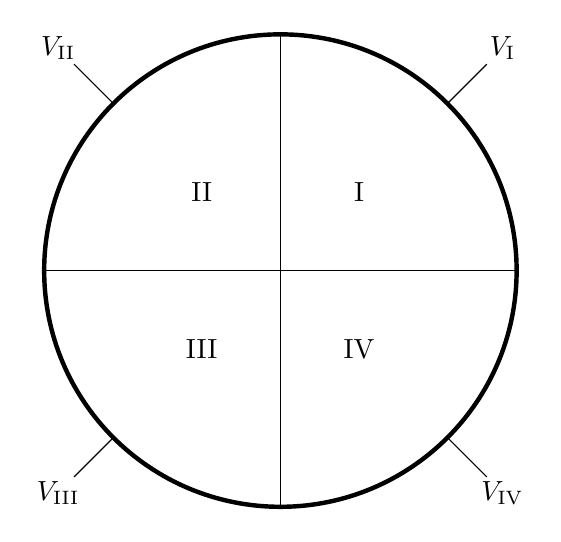
\begin{tikzpicture}
    \node (qpd) at (0,0){};
    \draw[ultra thick] (qpd) circle[radius=3cm];
    \draw (3cm,0cm) -- (-3cm,0cm);
    \draw (0cm,3cm) -- (0cm,-3cm);

    \node at (1cm, 1cm) {$\mathrm{I}$};
    \node at (-1cm, 1cm) {$\mathrm{II}$};
    \node at (1cm, -1cm) {$\mathrm{IV}$};
    \node at (-1cm, -1cm) {$\mathrm{III}$};

    \draw[thin] (2.1213203435596424cm,-2.1213203435596424cm) --++ (0.5cm,-0.5cm) node[xshift=0.2cm, yshift=-0.2cm]{$V_{\mathrm{IV}}$};
    \draw[thin] (2.1213203435596424cm,2.1213203435596424cm) --++ (0.5cm,0.5cm) node[xshift=0.2cm, yshift=0.2cm]{$V_{\mathrm{I}}$};
    \draw[thin] (-2.1213203435596424cm,2.1213203435596424cm) --++ (-0.5cm,0.5cm) node[xshift=-0.2cm, yshift=0.2cm]{$V_{\mathrm{II}}$};
    \draw[thin] (-2.1213203435596424cm,-2.1213203435596424cm) --++ (-0.5cm,-0.5cm) node[xshift=-0.2cm, yshift=-0.2cm]{$V_{\mathrm{III}}$};

    % \draw rectangle[width=2cm];
\end{tikzpicture}
\end{document}